\documentclass[../main.tex]{subfiles}

\begin{document}
	\section{Definizione}
	\label{sec:traformata_laplace}
	%schema a blocchi
	Operazione che consente di associare in modo \underline{biunivoco} ad una funzione $ f(t):\left[ 0^{-}, + \infty \right] $ un altra funzione $F(s)$ a valori complessi $ s = \sigma + j\omega \quad \sigma=\Re(s), \omega=\Im(s)$.\\
	%
	\linebreak
	Se l'integrale $ \int_{0^{-}}^{+\infty}f(t)e^{-st} \mathrm{d}t $ esiste (calcolabile finito), allora $f(t)$ è Laplace-trasformabile:
	$$ \Lbrace{f(t)} = F(s) = \LaplDef{f(t)}{s}{t} $$
	%
	\linebreak
	Si definisce \textbf{ascissa di convergenza} per la trasformata di Laplace di una funzione $f(t)$ la quantit\'a:\\
	$$ \bar{\sigma} \in \R \qquad \bar{\sigma} = inf\left\lbrace \Re{(s)} \colon \exists F(s) = \Lbrace{f(t)} \right\rbrace $$
	In parole povere si prendono tutti i numeri complessi per cui esiste la trasformata di Laplace. Quindi $ \bar{\sigma} $ è l'estremo inferiore di questo insieme (non \'e detto che sia anche il minimo).
	\begin{figure}[H]
		\centering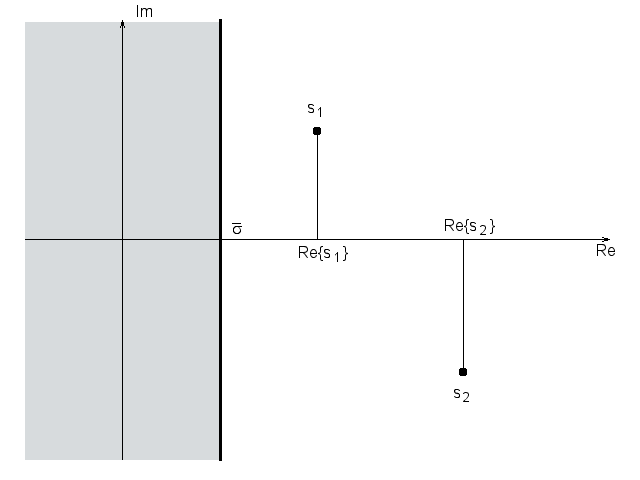
\includegraphics[width=.3\textwidth]{trasformata_laplace/ascissa_convergenza}
	\end{figure}
	%
	\paragraph{Teorema 1} Se la trasformata di Laplace esiste per qualche $s=\bar{s}$, allora essa esiste anche $ \forall s\ \text{tale che}\ \Re{(s)} > \Re{\bar{(s)}} $.\\
	$\rightarrow$ In pratica l'ascissa di convergenza definisce il limite a destra del quale la trasformata esiste sempre.
	%
	\paragraph{Teorema 2} La trasformata di Laplace \'{e} "analitica" $ \forall s \colon \Re{(s)} > \bar{\sigma}$. Analitica significa che \'e continua e derivabile $\infty$ volte.\\
	$\rightarrow$ In pratica, se una $f$ non \'e continua n\'e derivabile in alcuni punti, la sua trasformata lo \'e comunque: \'e pi\'u facile lavorare con quest'ultima.
	%	
	\section{Propriet\'{a}}
	%
	\subsection{Linearit\'{a}}
	\label{linear}
	$$ \Lapl{f_{1}(t)}{F_{1}(t)} \qquad \Lapl{f_{2}(t)}{F_{2}(t)} $$
	$$ \Rightarrow \Lapl{f(t)=\alpha f_{1}(t) + \beta f_{2}(t)}{F(s)=\alpha F_{1}(s) + \beta F_{2}(s)} $$
	Dimostrazione:
	\begin{align*}
		\Lbrace{f(t)} = F(s) &= \LaplDef{(\alpha f_{1}(t) + \beta f_{2}(t))}{s}{t} =\\
		&= \alpha \LaplDef{f_{1}(t)}{s}{t} + \beta \LaplDef{f_{2}(t)}{s}{t} = \alpha F_{1}(s) + \beta F_{2}(s)
	\end{align*}
	%
	\subsection{Traslazione in t}
	\label{trasl_t}
	$$ \Lapl{f(t)}{F(s)} \quad \Rightarrow \quad \Lapl{f(t-T)\ 1(t-T)}{e^{-sT}F(s)} $$
	\linebreak
	Dimostrazione: chiamiamo $ \bar{f}(t) = f(t-T)\ 1(t-T) $. Con il gradino non consideriamo tutto ci\'{o} che accade prima di $T$, altrimenti la trasformata sarebbe stata diversa e avrebbe incluso anche il tratto $(0^{-},+ \infty)$.
	\begin{align*}
		\Lbrace{\bar{f}(t)} &= \LaplDef{\bar{f}(t)}{s}{t} = \int_{0^{-}}^{T^{-}} \bar{f}(t) e^{-st} \mathrm{d}t + \int_{T^{-}}^{+ \infty} \bar{f}(t) e^{-st} \mathrm{d}t =\\
		&= 0+ \int_{T^{-}}^{+ \infty} f(t-T)\ 1\ e^{-st} \mathrm{d}t=
		&&\text{il gradino vale 1 in } (T^{-},+ \infty) \\
		&= \int_{0^{-}}^{+ \infty} f(\tau) e^{-s(\tau+T)} \mathrm{d}\tau = &&\text{ho cambiato variabile} \quad \tau=t-T\\
		&= e^{-sT} \LaplDef{f(\tau)}{s}{\tau} = e^{-sT} F(s)
	\end{align*}
	%
	\subsection{Traslazione in s}
	\label{trasl_s}
	$$ \Lapl{f(t)}{F(s)} \quad \Rightarrow \quad \Lapl{e^{at}f(t)}{F(s-a)}$$
	Dimostrazione: chiamo $\tilde{f}(t) = e^{at} f(t) $:\\
	\[
		\Lbrace{\tilde{f}(t)} = \LaplDef{\tilde{f}(t)}{s}{t} = \LaplDef{e^{at}f(t)}{s}{t} = \int_{0^{-}}^{+ \infty} f(t) e^{-(s-a)t} \mathrm{d}t = F(s-a)
	\]
	%
	\subsection{Derivata in t}
	\label{deriv_t}
	$$ \Lapl{f(t)}{F(s)} \quad \Rightarrow \quad \Lapl{\dot{f}(t)}{sF(s)-f(0^{-})} $$
	Dimostrazione:
	\begin{align*}
		\Lbrace{\dot{f}(t)} &= \LaplDef{\dot{f}(t)}{s}{t} \quad \rightarrow \text{Integro per parti} \rightarrow \left( \int f^{'}(x)g(x)\mathrm{d}x = f(x)g(x) - \int f(x)g^{'}(x) \mathrm{d}x \right)\\
		&= \left[ f(t)e^{-st} \right]_{0^{-}}^{+\infty} - \LaplDef{f(t)(-s)}{s}{t} =\\
		&= 0 - f(0^{-}) + s \LaplDef{f(t)}{s}{t} = sF(s)-f(0^{-})
	\end{align*}
	%
	\subsection{Derivata n-esima in t}
	\label{deriv_n_t}
	\begin{align*}
		\Lapl{g(t)=\dot{f}(t)}{&G(s) = sF(s) - f(0^{-})}\\
		\Lapl{\dot{g}(t) = \ddot{f}(t)}{&sG(s) - g(0^{-})}= \quad \text{Per la propriet\'{a} (\ref{deriv_t})} \quad
		=\ s[sF(s) - f(0^{-})] - \dot{f}(0^{-})\\
		\text{Quindi:} \quad \Lapl{\ddot{f}(t)}{&s^2 F(s) - s f(0^{-}) - \dot{f}(0^{-})} \\
		\text{Per } n=3 \text{:} \quad \Lapl{\frac{\mathrm{d^3}}{\mathrm{d}t^3}f(t)}{&s^3 F(s) - s^2 f(0^{-}) - s f^{(1)}(0^{-}) - f^{(2)}(0^{-})} \\
		\text{Per } n \text{:} \quad		\Lapl{\frac{\mathrm{d^n}}{\mathrm{d}t^n}f(t)}{&s^n F(s) - s^{n-1} f(0^{-}) - s^{n-2} f^{(1)}(0^{-}) -\ _{\dots}\ - s f^{(n-2)}(0^{-}) - f^{(n-1)}(0^{-})} = \\
		= &s^n F(s) - \sum_{k = 1}^{n} s^{n-k} f^{(k - 1)}(0^{-})
	\end{align*}
	%
	\subsection{Integrale in t}
	\label{int_t}
	$$ \Lapl{\int_{0^{-}}^{t} f(\tau) \mathrm{d}\tau}{\frac{1}{s} F(s)} $$
	%
	Dimostrazione:
	$$ g(t) = \int_{0^{-}}^{t} f(\tau) \mathrm{d}\tau \quad 		\dot{g}(t) = f(t) \quad g(0) = 0 $$
	Per la propriet\'{a} della derivata in t (\ref{deriv_t}):
	$$ 	F(s) = \Lbrace{f(t)} = \Lbrace{\dot{g}(t)} = s \Lbrace{g(t)} - g(0^{-}) = s G(s) - 0 \quad \Rightarrow \quad G(s) = \frac{1}{s} F(s) $$
	%
	\subsection{Derivata in s}
	\label{deriv_s}
	\begin{align*}
	\Lapl{t f(t)}{&- \frac{\mathrm{d}}{\mathrm{d}s} F(s)}\\
	\Lapl{t^n f(t)}{&(-1)^n \frac{\mathrm{d}^n}{\mathrm{d}s^n} F(s)}
	\end{align*}
	Dimostrazione ($n=1$): dalla definizione ho che:
	\[
		\frac{\mathrm{d}}{\mathrm{d}s} F(s) = \frac{\mathrm{d}}{\mathrm{d}s} \LaplDef{f(t)}{s}{t} =
	\]
	Uso la regola di derivazione sotto segno di integrale
	\[
		= \LaplDef{f(t) \pder{}{s}}{s}{t} = \LaplDef{f(t)(-t)}{s}{t} = - \LaplDef{t f(t)}{s}{t}=\Lbrace{t f(t)}
	\]
	%
	\section{Trasformate di funzioni notevoli}
	\subsection{Impulso}
	\label{trasf_impulso}
	Dalla definizione, per il campionamento:
	$$ \Lbrace{\delta (t)} = \LaplDef{\delta (t)}{s}{t} = \int_{0^{-}}^{+ \infty} \delta(t) \cdot 1 \mathrm{d}t = 1 $$
	%
	\subsection{Doppietto}
	\label{trasf_doppietto}
	Per la propriet\'{a} della derivata in t (\ref{deriv_t}):
	\begin{align*}
		\Lapl{\dot{\delta}(t)}{&s\ \Lbrace{\delta(t)} - \delta(0^-) = s}\\
		\Lapl{\delta^{(n)}(t)}{&s^n} \qquad \text{se tutte le condizioni iniziali sono nulle}
	\end{align*}
	%
	\subsection{Gradino}
	\label{trasf_gradino}
	Calcoliamo con due metodi differenti:
	\begin{enumerate}
		\item Utilizziamo la definizione:
		\[\LaplDef{1(t)}{s}{t} = \LaplDef{}{s}{t} = -\frac{1}{s}\ \left[ e^{-st} \right]_{0^-}^{+ \infty} = -\frac{1}{s} (-1) = \frac{1}{s}\]
		\item \'{E} l'integrale del gradino, quindi possiamo utilizzare la propriet\'{a} (\ref{int_t}):
		$$ 1(t) = \int_{0^-}^{t} \delta(\tau) \mathrm{d}\tau $$
		$$ \text{Allora:} \qquad \Lapl{1(t)}{\frac{1}{s}\ \Lbrace{\delta(t)} = \frac{1}{s}} $$
	\end{enumerate}
	%
	\subsection{Rampa}
	\label{trasf_rampa}
	\'{E} l'integrale del gradino, quindi utilizziamo la propriet\'{a} (\ref{int_t}):
	\begin{align*}
		\Lapl{t\ 1(t)}{&\frac{1}{s} \Lbrace{1(t)}} = \frac{1}{s^2}
		\intertext{Generalizziamo per il grado n:}
		\Lapl{t^n 1(t)}{&n! \frac{1}{s^{n+1}}}
	\end{align*}
	%
	\subsection{Esponenziale}
	\label{trasf_esponenziale}
	Trasformando un esponenziale si ottiene un ritardo:
	$$ \Lapl{e^{\sigma t}\ 1(t)}{\frac{1}{s-\sigma}} $$
	%
	\subsection{Alcune $f$ composte: Polinomio ed Esponenziale}
	Partiamo dal grado 1: $ \qquad t\ e^{\sigma t} 1(t) = t\ f(t) $
	\begin{align*}
		\text{Per la propriet\'{a} (\ref{deriv_s}):} \qquad \Lapl{t\ f(t)}{&(-1) \der{}{s} F(s)}\\
		%
		\text{Quindi:} \qquad \Lapl{f(t) = e^{\sigma t} 1(t)}{&F(s) = \frac{1}{s-\sigma}}\\
		%
		\Rightarrow \quad \Lapl{t e^{\sigma t} 1(t)}{&(-1) \der{}{s} \frac{1}{s-\sigma}} = (-1) \frac{-1}{(s-\sigma)^2} = \frac{1}{(s-\sigma)^2}
	\end{align*}
		Generalizziamo al grado $n$: \quad chiamo \quad $f(t) = t^n 1(t)$\\
		Quindi per la presenza dell'esponenziale sto effettuando una traslazione in s:
		\[
			\Lapl{e^{\sigma t} f(t)}{F(s-\sigma) = n! \frac{1}{(s-\sigma)^{n+1}}}
		\]
	%
	\subsection{Seno}
	\label{trasf_seno}
	Scriviamo il seno attraverso la rappresentazione di Eulero dei numeri complessi:
	\begin{align*}
		\Lbrace{\sin(wt) 1(t)} &= \Lbrace{\frac{e^{jwt} - e^{-jwt}}{2j} 1(t)} =\\
		&= \frac{1}{2j} \left[ \Lbrace{e^{jwt} 1(t)} - \Lbrace{e^{-jwt} 1(t)} \right]= \qquad &&\text{per linearit\'{a}}\\
		&= \frac{1}{2j} \left[ \frac{1}{s-jw} - \frac{1}{s-(-jw)} \right] = \qquad &&\text{traslazione in s}\\
		&= \frac{1}{2j} \frac{s+jw-s+jw}{s^2+w^2} = \frac{w}{s^2+w^2}
	\end{align*}
	%
	\subsection{Coseno}
	\label{trasf_coseno}
	\begin{align*}
		\Lbrace{\cos(wt) 1(t)} &= \Lbrace{\frac{e^{jwt} + e^{-jwt}}{2} 1(t)} =\\
		&= \frac{1}{2} \left[ \Lbrace{e^{jwt} 1(t)} + \Lbrace{e^{-jwt} 1(t)} \right] =\\
		&= \frac{1}{2} \left[ \frac{1}{s+jw} + \frac{1}{s-jw} \right] =\\
		&= \frac{1}{2} \left[ \frac{s-jw+s+jw}{s^2+w^2} \right] = \frac{s}{s^2+w^2} \\
	\end{align*}
	%
	\subsection{Seno e Coseno (2)}
	Gli stessi risultati possono essere ottenuti sfruttando la propriet\'{a} (\ref{deriv_t}) di derivazione in t.\\
	\rule{\linewidth}{0.4pt}
	Ad esempio partiamo dal seno:
	$$ \sin(wt) \quad \xrightarrow{\der{}{t}} \quad w \cos(wt) \quad \xrightarrow{\der{}{t}} \quad -w^2 \sin(wt) $$
	Conosciamo la trasformata della funzione seno:
	$$ \Lbrace{\sin(wt)} = \frac{w}{s^2+w^2} $$
	Calcoliamo la trasformata della sua derivata:
	$$ w \cos(wt) = \der{}{t} \sin(wt) \quad\Rightarrow\quad \Lbrace{w \cos(wt)} = \Lbrace{\der{}{t} \sin(wt)} $$
	$$ \Lbrace{\der{}{t} \sin(wt)} = s \frac{w}{s^2+w^2} - \sin(w\ 0^-) = \frac{sw}{s^2+w^2} $$
	Poich\'{e} la trasformata di Laplace \'{e} lineare (\ref{linear}) otteniamo la stessa trasformata del coseno calcolata in precedenza.
	$$ \Rightarrow \quad \frac{1}{w} \cdot \Lbrace{w\cos(wt)} = \frac{sw}{s^2+w^2} \cdot \frac{1}{w} = \frac{s}{s^2+w^2} $$
	Calcoliamo la trasformata della derivata seconda del seno:
	$$ -w^2 \sin(wt) = \der{}{t} w\cos(wt) \quad\Rightarrow\quad \Lbrace{-w^2 \sin(wt)} = \Lbrace{\der{}{t} w\cos(wt)} $$
	$$ \Lbrace{\der{}{t} w\cos(wt)} = s \frac{sw}{s^2+w^2} - w\cos(w\ 0^-) = \frac{s^2w}{s^2+w^2} - w = \frac{-w^3}{s^2+w^2}$$
	$$ \Rightarrow \quad \left( - \frac{1}{w^2} \right) \cdot \Lbrace{-w^2 \sin(wt)} = \left[ \frac{-w^3}{s^2+w^2} \right] \cdot \left( - \frac{1}{w^2} \right) = \frac{w}{s^2+w^2} $$
	\rule{\linewidth}{0.4pt}
	Analogamente partendo dal coseno:
	$$ \cos(wt) \quad \xrightarrow{\der{}{t}} \quad -w\sin(wt) \quad \xrightarrow{\der{}{t}} \quad -w^2\cos(wt) $$	
	Calcoliamo la trasformata della sua derivata:
	$$ -w\sin(wt) = \der{}{t} \cos(wt) \quad\Rightarrow\quad \Lbrace{-w\sin(wt)} = \Lbrace{\der{}{t} \cos(wt)} $$
	$$ \Lbrace{\der{}{t} \cos(wt)} = s \frac{s}{s^2+w^2} - \cos(w\ 0^-) = \frac{s^2}{s^2+w^2} - 1 $$
	$$ \Rightarrow \quad -\frac{1}{w} \cdot \Lbrace{-w\sin(wt)} = \left[ \frac{s^2}{s^2+w^2} - 1 \right] \cdot \left( -\frac{1}{w}\right) = \left[ \frac{s^2-s^2-w^2}{s^2+w^2} \right] \cdot \left( -\frac{1}{w}\right) = \frac{w}{s^2+w^2} $$
	Calcoliamo la trasformata della derivata seconda del coseno:
	$$ -w^2 \cos(wt) = \der{}{t} \left[ -w\sin(wt) \right] \quad\Rightarrow\quad \Lbrace{-w^2 \cos(wt)} = \Lbrace{\der{}{t} \left[ -w\sin(wt) \right]} $$
	$$ \Lbrace{\der{}{t} \left[ -w\sin(wt) \right]} = s \left[ \frac{s^2}{s^2+w^2} - 1 \right] - \left[ -w\sin(w\ 0^-) \right] = s \left[ \frac{s^2}{s^2+w^2} - 1 \right] $$
	$$ \Rightarrow \quad \left( - \frac{1}{w^2} \right) \cdot \Lbrace{-w^2 \cos(wt)} = s \left[ \frac{s^2}{s^2+w^2} - 1 \right] \left[ - \frac{1}{w^2} \right] = \left[ \frac{\not{s^2}-\not{s^2}-w^2}{s^2+w^2} \right] \left[ -\frac{s}{w^2} \right] = \frac{s}{s^2+w^2} $$
	%
	\subsection{Polinomio e seno}
	\label{trasf_t_seno}
	Vogliamo calcolare la trasformata di: $$ t \cdot \sin(wt) \cdot 1(t) $$
	Chiamo: $$ f(t) = \sin(wt)1(t) $$
	Allora posso applicare la propriet\'{a} (\ref{deriv_s}) della derivata in s: $$ \Lapl{t f(t)}{-\der{}{s}\left( \frac{w}{s^2+w^2}\right) = \frac{2ws}{(s^2+w^2)^2}} $$
	%
	\subsection{Polinomio e coseno}
	\label{trasf_t_coseno}
	Vogliamo calcolare la trasformata di: $$ t \cdot \cos(wt) \cdot 1(t) $$
	Chiamo: $$ f(t) = \cos(wt)1(t) $$
	Allora posso applicare la propriet\'{a} (\ref{deriv_s}) della derivata in s: $$ \Lapl{t f(t)}{-\der{}{s}\left( \frac{s}{s^2+w^2}\right) = -\frac{s^2+w^2-s(2s)}{(s^2+w^2)^2}} = \frac{s^2-w^2}{(s^2+w^2)^2} $$
	%
	\subsection{Esponenziale e seno}
	Grazie alla propriet\'{a} (\ref{trasl_s}) di traslazione in s:
	$$ \Lapl{e^{\sigma t} \sin(wt) 1(t)}{ \left. \frac{w}{\bar{s}^2+w^2} \right|_{\bar{s}=s-\sigma} = \frac{w}{(s-\sigma)^2 + w^2}} $$
	%
	\subsection{Esponenziale e coseno}
	Grazie alla propriet\'{a} (\ref{trasl_s}) di traslazione in s:
	$$ \Lapl{e^{\sigma t} \cos(wt) 1(t)}{ \left. \frac{\bar{s}}{\bar{s}^2+w^2} \right|_{\bar{s}=s-\sigma} = \frac{s-\sigma}{(s-\sigma)^2 + w^2}} $$
	%
	\subsection{Polinomio grado 1, esponenziale e seno}
	Utilizziamo la propriet\'{a} della derivata in s (\ref{deriv_s}):
	$$ \Lbrace{t\ e^{\sigma t} \sin(wt) 1(t)} = t f(t) = -\der{}{s} \left( \frac{w}{(s-\sigma)^2+w^2} \right) = - \left[ -\frac{w\ 2(s-\sigma)}{[(s-\sigma)^2+w^2]^2} \right] = \frac{2w(s-\sigma)}{[(s-\sigma)^2+w^2]^2} $$
	%
	\subsection{Polinomio grado 2, esponenziale e seno}
	\begin{enumerate}
		\item utilizziamo la propriet\'{a} di derivazione in s:
		$$ t^2\ e^{\sigma t} \sin(wt) 1(t) = t\ f(t) $$
		Ma questo metodo comporta il calcolo della derivata della trasformata trovata nel paragrafo precedente e potrebbe essere un po' complicato.
		\item utilizziamo la propriet\'{a} della traslazione in s (\ref{trasl_s}):
		$$ t^2\ e^{\sigma t} \sin(wt) 1(t) = e^{\sigma t} f(t) $$
		\begin{align*}
		\Lbrace{f(t)} &= \Lbrace{t^2\ \sin(wt) 1(t)} = \Lbrace{t \cdot (t\ \sin(wt) 1(t))} =\\
		&= -\der{}{s} \left( \frac{2ws}{(s^2+w^2)^2} \right) = -\frac{2w(s^2+w^2)^2-2ws \cdot 2(s^2+w^2) \cdot 2s}{(s^2+w^2)^4} =\\ 
		&= -2w \frac{s^2+w^2-4s^2}{(s^2+w^2)^3} = 2w \frac{3s^2-w^2}{[s^2+w^2]^3}
		\end{align*}
		$$ \Rightarrow \Lbrace{e^{\sigma t} f(t)} = 2w \frac{3(s-\sigma)^2 - w^2}{[(s-\sigma)^2+w^2]^3} $$
	\end{enumerate}
	%
	\subsection{Polinomio grado 1, esponenziale e coseno}
	Utilizziamo la propriet\'{a} della derivata in s (\ref{deriv_s}):
	\[
	 	\Lbrace{t\ e^{\sigma t} \cos(wt) 1(t)} = t f(t) = -\der{}{s} \left( \frac{s-\sigma}{(s-\sigma)^2+w^2} \right) =
	 \]
	 \[	
	 	=-\frac{(s-\sigma)^2+w^2-2(s-\sigma)(s-\sigma)}{[(s-\sigma)^2+w^2]^2} = \frac{(s-\sigma)^2-w^2}{[(s-\sigma)^2+w^2]^2}
	 \]
	\subsection{Polinomio grado 2, esponenziale e coseno}
	\begin{enumerate}
		\item utilizziamo la propriet\'{a} di derivazione in s (\ref{deriv_s}):
		$$ t^2\ e^{\sigma t} \cos(wt) 1(t) = t\ f(t) $$
		Ma questo metodo comporta il calcolo della derivata della trasformata trovata nel paragrafo precedente e potrebbe essere un po' complicato.
		\item utilizziamo la propriet\'{a} della traslazione in s (\ref{trasl_s}):
		$$ t^2\ e^{\sigma t} \cos(wt) 1(t) = e^{\sigma t} f(t) $$
		\begin{align*}
		\Lbrace{f(t)} &= \Lbrace{t^2\ \cos(wt) 1(t)} = \Lbrace{t \cdot (t\ \cos(wt) 1(t))} =\\
		&= -\der{}{s} \left( \frac{s^2-w^2}{(s^2+w^2)^2} \right) = -\frac{2s(s^2+w^2)^2 - (s^2-w^2) \cdot 2 \cdot (s^2+w^2) \cdot 2s}{(s^2+w^2)^4} =\\ 
		&= -\frac{2s}{(s^2+w^2)^3} \left[ s^2+w^2-2s^2+2w^2 \right] = \frac{2s^3-6w^2s}{[s^2+w^2]^3}
		\end{align*}
		$$ \Rightarrow \Lbrace{e^{\sigma t} f(t)} = \frac{2(s-\sigma)^3-6w^2(s-\sigma)}{[(s-\sigma)^2+w^2]^3} $$
	\end{enumerate}
	%
	\subsection{Prodotto di convoluzione: definizione}
	\begin{equation}
		f(t) * g(t) = \int_{0}^{t} f(\tau)g(t-\tau) d\tau \quad \text{se}\ f(t), g(t)\ \text{nulle}\ \forall t
	\end{equation}
	\paragraph{Significato}
	\begin{enumerate}
		\item Supponiamo di fissare il tempo in un certo istante $\bar{t}$
		\item Ribaltiamo $g(t)$ rispetto l'asse verticale e lo trasliamo in $\bar{t}$
		\item Calcoliamo l'integrale da 0 a $\bar{t}$ di $f(\bar{t})g(\bar{t}-\tau)$, cio\'{e} l'area sottesa dal prodotto dalle funzioni
		\item Ripetiamo il procedimento per ogni $\bar{t}$ e otteniamo una funzione che associa ad ogni istante di tempo il valore di quell'integrale
	\end{enumerate}
	\'{E} facile dimostrare che vale la propriet\'{a} \textbf{commutativa} attraverso un cambio di variabili. \label{conv_comm}
	$$ \int_{0}^{t} f(\tau)g(t-\tau) d\tau = \int_{0}^{t} g(\tau)f(t-\tau) d\tau $$
	$$ f(t)*g(t) = g(t)*f(t) $$
	%
	\subsection{Prodotto di convoluzione: trasformata}
	$$ \text{Se} \quad \Lapl{f(t)}{F(s)} \qquad \Lapl{g(t)}{G(s)} $$
	$$ \text{allora} \quad \Lapl{f(t)*g(t)}{F(s)G(s)} $$
\end{document}